\documentclass[12pt,a4paper,oldfontcommands]{memoir}
\usepackage[utf8]{inputenc}
\usepackage[T1]{fontenc}
\usepackage{microtype}
\usepackage[dvips]{graphicx}
\usepackage{xcolor}
\usepackage{times}

\usepackage[
breaklinks=true,colorlinks=true,
%linkcolor=blue,urlcolor=blue,citecolor=blue,% PDF VIEW
linkcolor=black,urlcolor=black,citecolor=black,% PRINT
bookmarks=true,bookmarksopenlevel=2]{hyperref}

\usepackage{biblatex}
\addbibresource{sample.bib}


\usepackage{geometry}
% PDF VIEW
% \geometry{total={210mm,297mm},
% left=25mm,right=25mm,%
% bindingoffset=0mm, top=25mm,bottom=25mm}
% PRINT
\geometry{total={210mm,297mm},
left=20mm,right=20mm,
bindingoffset=10mm, top=25mm,bottom=25mm}

\OnehalfSpacing
%\linespread{1.3}

%%% CHAPTER'S STYLE
%\chapterstyle{bianchi}
%\chapterstyle{ger}
\chapterstyle{madsen}
%\chapterstyle{ell}
%%% STYLE OF SECTIONS, SUBSECTIONS, AND SUBSUBSECTIONS
\setsecheadstyle{\Large\bfseries\sffamily\raggedright}
\setsubsecheadstyle{\large\bfseries\sffamily\raggedright}
\setsubsubsecheadstyle{\bfseries\sffamily\raggedright}


%%% STYLE OF PAGES NUMBERING
%\pagestyle{companion}\nouppercaseheads 
%\pagestyle{headings}
%\pagestyle{Ruled}
\pagestyle{plain}
\makepagestyle{plain}
\makeevenfoot{plain}{\thepage}{}{}
\makeoddfoot{plain}{}{}{\thepage}
\makeevenhead{plain}{}{}{}
\makeoddhead{plain}{}{}{}


\maxsecnumdepth{subsection} % chapters, sections, and subsections are numbered
\maxtocdepth{subsection} % chapters, sections, and subsections are in the Table of Contents


%%%---%%%---%%%---%%%---%%%---%%%---%%%---%%%---%%%---%%%---%%%---%%%---%%%

\begin{document}

%%%---%%%---%%%---%%%---%%%---%%%---%%%---%%%---%%%---%%%---%%%---%%%---%%%
%   TITLEPAGE
%
%   due to variety of titlepage schemes it is probably better to make titlepage manually
%
%%%---%%%---%%%---%%%---%%%---%%%---%%%---%%%---%%%---%%%---%%%---%%%---%%%
\thispagestyle{empty}

{%%%
\sffamily
\centering
\Large

~\vspace{\fill}

{\huge 
Thesis title: may be long or short
}

\vspace{2.5cm}

{\LARGE
Your name
}

\vspace{3.5cm}

A thesis submitted in partial fulfillment for the\\
degree of Doctor of Philosophy\\[1em]
in the\\[1em]
Faculty Name\\
University Name

\vspace{3.5cm}

Supervisor: Prof. Joe Doe

\vspace{\fill}

May 2013

%%%
}%%%

\cleardoublepage
%%%---%%%---%%%---%%%---%%%---%%%---%%%---%%%---%%%---%%%---%%%---%%%---%%%
%%%---%%%---%%%---%%%---%%%---%%%---%%%---%%%---%%%---%%%---%%%---%%%---%%%

\tableofcontents*

\newpage
\listoffigures

\clearpage

%%%---%%%---%%%---%%%---%%%---%%%---%%%---%%%---%%%---%%%---%%%---%%%---%%%
%%%---%%%---%%%---%%%---%%%---%%%---%%%---%%%---%%%---%%%---%%%---%%%---%%%

\chapter{INTRODUCTION}

\section{Content}
Natural Language Processing(NLP) is an area of research and application that explores how computers can be used to understand and manipulate natural language text or speech to do useful things. NLP researchers aim to gather knowledge on how human beings understand and use language so that appropriate tools and techniques can be developed to make computer systems understand and manipulate natural languages to perform the desired tasks. The foundations of NLP lie in a number of disciplines, viz. computer and information sciences, linguistics, mathematics, electrical and electronic engineering, artificial intelligence and robotics, psychology, etc. Applications of NLP include a number of fields of studies, such as machine translation, natural language text processing and summarization, user interfaces, multilingual and cross language information retrieval(CLIR), speech recognition, artificial intelligence and expert systems, and so on\cite1.

At the core of any NLP task there is the important issue of natural language understanding. The process of building computer programs that understand natural language involves three major problems: the first one relates to the thought process, the second one to the representation and meaning of the linguistic input, and the third one to the world knowledge. Thus, an NLP system may begin at the word level – to determine the morphological structure, nature(such as part-of- speech, meaning) etc. of the word – and then may move on to the sentence level – to determine morphological level that deals with the smallest parts of words, that carry a meaning, and suffixes and prefixes:-  lexical level that deals with lexical meaning of words and parts of speech analyses, syntactic level that deals with grammar and structure of sentences, semantic level that deals with the meaning of words and sentences, discourse level that deals with the structure of different kinds of text using document structures and pragmatic level that deals with the knowledge that comes from the outside world, i.e. from outside the contents of the document.

The goal of automatic speech recognition is to develop technique and system that enables computers to accept speech input. NLP is a field of computer science and linguistics concerned with the interactions between computers and human(natural) languages. In theory, natural-language processing is a very attractive method of human-computer interaction. Natural-language understanding is sometimes referred to as an AI-complete problem, because natural-language recognition seems to require extensive knowledge about the outside world and the ability to manipulate it.

NLP is an area of research and application that explores how computers can be used to understand and manipulate natural language text or speech to do useful things. NLP researchers aim to gather knowledge on how human beings understand and use language so that appropriate tools and techniques can be developed to make computer systems understand and manipulate natural languages to perform the desired tasks. The foundations of NLP lie in a number of disciplines, disciplines, viz. computer and information sciences, linguistics, mathematics, electrical and electronic engineering, artificial intelligence and robotics, psychology, etc.Research in natural language processing has been going on for several decades dating back to the late 1940s. Machine translation(MT) was the first computer-based application related to natural language.

Natural language processing approaches fall roughly into four categories: symbolic, statistical, connectionist, and hybrid. Symbolic and statistical approaches have coexisted since the early days of this field. Connectionist NLP work first appeared in the 1960’s. For a long time, symbolic approaches dominated the field. In the 1980’s, statistical approaches regained popularity as a result of the availability of critical computational resources and the need to deal with broad, real- world contexts. Connectionist approaches also recovered from earlier criticism by demonstrating the utility of neural networks in NLP.

Speech is a complex phenomenon. It is important to  understand how is it produced and perceived. The naive perception is often that speech is built with words, and each word consists of phones. The reality is unfortunately very different. Speech is a dynamic process without clearly distinguished parts.

\subsection{Structure of speech}
Speech is a continuous audio stream where rather stable states mix with dynamically changed states. In this sequence of states, one can define more or less similar classes of sounds, or \textbf{phones}. Words are understood to be built of phones, but this is certainly not true. The acoustic properties of a waveform corresponding to a phone can vary greatly depending on many factors - phone context, speaker, style of speech and so on. The so called coarticulation makes phones sound very different from their “canonical” representation. Next, since transitions between words are more informative than stable regions, developers often talk about \textbf{diphones}- parts of phones between two consecutive phones. Sometimes developers talk about subphonetic units - different substates of a phone. Often three or more regions of a different nature can easily be found.

The first part of the phone depends on its preceding phone, the middle part is stable, and the next part depends on the subsequent phone. That's why there are often three states in a phone selected for speech recognition.Sometimes phones are considered in context. Such phones in context are called \textbf{triphones} or even \textbf{quinphones}. For computational purpose it is helpful to detect parts of triphones instead of triphones as a whole, for example, to create a detector for a beginning of triphone and share it across many triphones. The whole variety of sound detectors can be represented by a small amount of distinct short sound detectors. Usually we use 4000 distinct short sound detectors to compose detectors for triphones. We call those detectors \textbf{senones}. 

\section{ Problem Statement}

In this thesis work, the problem formulation for Punjabi Dictation in Natuarl Language Processing is defined. It would lead to the development of the system for the Punjab language model and Gurmuki font so that the speech to text covergence softwares and systems could convert speech data into Gurmukhi font. As the speech to text convergence is available for the some internationl language, but are not available for punjabi language and Gurmukhi font. The model used for this purpose is HMM(Hidden Markov’s MOdel) along with the CMUSphinx toolkit which are responsible for speech recognization and storing the data to the database. Further many liberaries are available for defining the new Acoustic Model for the different languages, so, we would use one of these model for defining language model for our requirement. The output of the data may be extracted through terminal using ANSI terminal protocol.

\section{Aims and Objectives}

\begin{description}
  \item[$\bullet$] Our main objective is to develop an application for Punjabi Dictation.
  \item[$\bullet$] Make decision about the use of specific library and software.
  \item[$\bullet$] Construct database for the words in Punjabi. 
  \item[$\bullet$] Construct database for the speech in Punjabi. 
  \item[$\bullet$] Develop a Language Model for Punjabi language.	
\end{description}

\section{Organization of the Thesis}
The reminder of thesis is organized as:

In \textbf{Chapter 2}, we need to have introduction of fundamentals of Speech recognition and Dictation and its challenges. Also characteristics, advantages of Speech-to-Text are discussed. Dictation performance and issues are described. Then CMUSphinx, Hidden Markov's Model are described.\\

In \textbf{Chapter 3}, we cover the literature review of our topic.\\


In \textbf{Chapter 4}, we cover the proposed scheme of our topic which includes motivation and basic design of our that are related to our topic.\\


In \textbf{Chapter 5}, we deal with experimental results and analysis of our work. This section describes the tools and platform used in our project.
The tool used in our project is CMULTK and plate form used is Linux and operating system is UBUNTU 14.04.\\


In \textbf{Chapter 6}, covers the conclusion by us. At last we have shown different references including research papers, websites and books which we have gone through during my projects. 




Citation of Einstein paper~\cite1





%===================================================================================================================================================






\chapter{ CONCEPTS OF SPEECH}

\section{Introduction}
Speech is a complex phenomenon. People rarely understand how is it produced and perceived. The naive perception is often that speech is built with words, and each word consists of phones. The reality is unfortunately very different. Speech is a dynamic process without clearly distinguished parts. It's always useful to get a sound editor and look into the recording of the speech and listen to it. Here is for example the speech recording in an audio editor.

\begin{figure}[h]
    \centering
    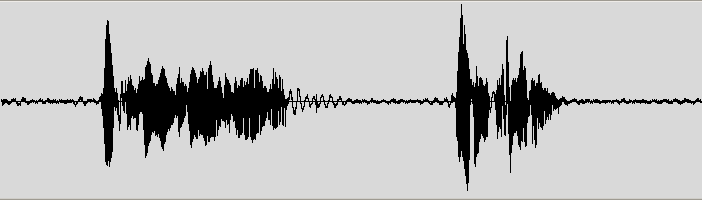
\includegraphics[scale=0.5]{waveform}
    \caption{Speech Waveform}
%    \label{fig:mesh1}
\end{figure}

All modern descriptions of speech are to some degree probabilistic. That means that there are no certain boundaries between units, or between words. Speech to text translation and other applications of speech are never 100 percent correct. That idea is rather unusual for software developers, who usually work with deterministic systems. And it creates a lot of issues specific only to speech technology. 


\subsection{Concept of speech}
Speech is a continuous audio stream where rather stable states mix with dynamically changed states. In this sequence of states, one can define more or less similar classes of sounds, or \textbf{phones}. Words are understood to be built of phones, but this is certainly not true. The acoustic properties of a waveform corresponding to a phone can vary greatly depending on many factors - phone context, speaker, style of speech and so on. The so called coarticulation makes phones sound very different from their “canonical” representation. Next, since transitions between words are more informative than stable regions, developers often talk about \textbf{diphones}- parts of phones between two consecutive phones. Sometimes developers talk about subphonetic units - different substates of a phone. Often three or more regions of a different nature can easily be found.

The first part of the phone depends on its preceding phone, the middle part is stable, and the next part depends on the subsequent phone. That's why there are often three states in a phone selected for speech recognition.Sometimes phones are considered in context. Such phones in context are called \textbf{triphones} or even \textbf{quinphones}. For computational purpose it is helpful to detect parts of triphones instead of triphones as a whole, for example, to create a detector for a beginning of triphone and share it across many triphones. The whole variety of sound detectors can be represented by a small amount of distinct short sound detectors. Usually we use 4000 distinct short sound detectors to compose detectors for triphones. We call those detectors \textbf{senones}. 


\subsection{Recognition precess}
 The common way to recognize speech is the following: we take waveform, split it on utterances by silences then try to recognize what's being said in each utterance. To do that we want to take all possible combinations of words and try to match them with the audio. We choose the best matching combination. There are few important things in this match.

First of all it's a concept of features. Since number of parameters is large, we are trying to optimize it. Numbers that are calculated from speech usually by dividing speech on frames. Then for each frame of length typically 10 milliseconds we extract 39 numbers that represent the speech. That's called eature vector. They way to generates numbers is a subject of active investigation, but in simple case it's a derivative from spectrum.

Second it's a concept of the model. Model describes some mathematical object that gathers common attributes of the spoken word. In practice, for audio model of senone is gaussian mixture of it's three states - to put it simple, it's a most probable feature vector. From concept of the model the following issues raised - how good does model fits practice, can model be made better of it's internal model problems, how adaptive model is to the changed conditions.

The model of speech is called \underline{Hidden Markov Model} or HMM, it's a generic model that describes black-box communication channel. In this model process is described as a sequence of states which change each other with certain probability. This model is intended to describe any sequential process like speech. It has been proven to be really practical for speech decoding.

Third, it's a matching process itself. Since it would take a huge time more than universe existed to compare all feature vectors with all models, the search is often optimized by many tricks. At any points we maintain best matching variants and extend them as time goes producing best matching variants for the next frame.

\subsubsection{Models}
According to the speech structure, three models are used in speech recognition to do the match:
\begin{description}
%  \item[$\cdot$ bla1] item 1
  \item[$\bullet$ Acoustic Model] contains acoustic properties for each senone. There are context-independent models that contain properties (most probable feature vectors for each phone) and context-dependent ones (built from senones with context). 
%  \item[$\ast$ bla3] item 3
  \item[$\bullet$ Phonetic Dictionary]
contains a mapping from words to phones. This mapping is not very effective. For example, only two to three pronunciation variants are noted in it, but it's practical enough most of the time. The dictionary is not the only variant of mapper from words to phones. It could be done with some complex function learned with a machine learning algorithm. 

  \item[$\bullet$ Language Model]
	s used to restrict word search. It defines which word could follow previously recognized words (remember that matching is a sequential process) and helps to significantly restrict the matching process by stripping words that are not probable. Most common language models used are n-gram language models-these contain statistics of word sequences-and finite state language models-these define speech sequences by finite state automation, sometimes with weights. To reach a good accuracy rate, your language model must be very successful in search space restriction. This means it should be very good at predicting the next word. A language model usually restricts the vocabulary considered to the words it contains. That's an issue for name recognition. To deal with this, a language model can contain smaller chunks like subwords or even phones. Please note that search space restriction in this case is usually worse and corresponding recognition accuracies are lower than with a word-based language model.

\end{description}

\begin{figure}[h]
    \centering
    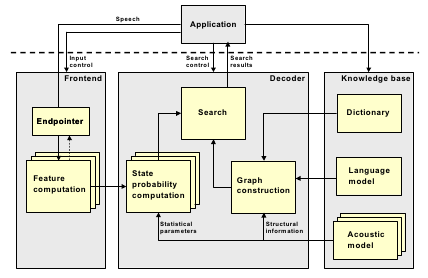
\includegraphics[scale=1.0]{sphinx4_architecture}
    \caption{Sphinx Architecture}
%    \label{fig:mesh1}
\end{figure}


Most current speech recognition systems use hidden Markov models(HMMs) to deal with the temporal variability of speech and Gaussian mixture models(GMMs) to deter- mine how well each state of each HMM fits a frame or a short window of frames of coefficients that repre- sents the acoustic input. An alternative way to evaluate the fit is to use a feed-forward neural network that takes several frames of coefficients as input and produces posterior probabilities over HMM states as output.

PocketSphinx is a flexible, modular and pluggable framework to help foster new innovations in the core research of hidden Markov model(HMM) speech recognition systems. The design of PocketSphinx is based on patterns that have emerged from the design of past systems as well as new requirements based on areas that researchers currently want to explore. To exercise this framework, and to provide researchers with a “research- ready” system, Sphinx-4 also includes several implementations of both simple and state-of-the-art techniques. The framework and the implementations are all freely available via open source.

PocketSphinx is a flexible, modular and pluggable framework to help foster new innovations in the core research of hidden Markov model (HMM) speech recognition systems. The design of PocketSphinx is based on patterns that have emerged from the design of past systems as well as new requirements based on areas that researchers currently want to explore. To exercise this framework, and to provide researchers with a “research- ready” system, Sphinx-4 also includes several implementations of both simple and state-of-the-art techniques. The framework and the implementations are all freely available via open source.

When researchers approach the problem of core speech recognition research, they are often faced with the problem of needing to develop an entire system from scratch, even if they only want to explore one facet of the field. Open source speech recognition systems are available, such as HTK , ISIP , AVCSR  and earlier versions of the Sphinx systems. The available systems are typically optimized for a single approach to speech system design. As a result, these systems intrinsically create barriers to future research that departs from the original purpose of the system.  First and foremost, PocketSphinx is a modular and pluggable framework that incorporates design patterns from existing systems, with sufficient flexibility to support emerging areas of research interest. The framework is modular in that it comprises separable components dedicated to specific tasks, and it is pluggable in that modules can be easily replaced at run time. To exercise the framework, and to provide researchers with a working system, PocketSphinx also includes a variety of modules that implement state-of-the-art speech recognition techniques.


\section{Advantages of Speech Recognition and Dictation systems}

\begin{description}
  \item[$\bullet$] Speech is a very natural way to interact, and it is not necessary to sit at a keyboard or work with a remote control.
  \item[$\bullet$] No training required for users.
  \item[$\bullet$] With speech recognition software, become a lot more productive – you’ll be able to get your work done much more quickly.
  \item[$\bullet$] Most of us can dictate at least 3 times faster than we can type. 
  \item[$\bullet$] It’s like having your own Personal Assistant available 24/7.	
\end{description}

\section{Principles of HMM}
Speech recognition systems generally assume that the speech signal is a realisation of some mes-sage encoded as a sequence of one or more symbols. To effect the reverse operation of recognising the underlying symbol sequence given a spoken utterance, the continuous speech waveform is first converted to a sequence of equally spaced discrete parameter vectors. This sequence of parameter vectors is assumed to form an exact representation of the speech waveform on the basis that for the duration covered by a single vector (typically 10ms or so), the speech waveform can be regarded as being stationary. Although this is not strictly true, it is a reasonable approximation. Typical parametric representations in common use are smoothed spectra or linear prediction coefficients plus various other representations derived from these. 

The role of the recogniser is to effect a mapping between sequences of speech vectors and the wanted underlying symbol sequences. Two problems make this very difficult. Firstly, the mapping from symbols to speech is not one-to-one since different underlying symbols can give rise to similar speech sounds. Furthermore, there are large variations in the realised speech waveform due to speaker variability, mood, environment, etc.  Secondly, the boundaries between symbols cannot be identified explicitly from the speech waveform. Hence, it is not possible to treat the speech waveform as a sequence of concatenated static patterns. 

The second problem of not knowing the word boundary locations can be avoided by restricting the task to isolated word recognition. This implies that the speech waveform corresponds to a single underlying symbol (e.g. word) chosen from a fixed vocabulary. Despite the fact that this simpler problem is somewhat artificial, it nevertheless has a wide range of practical applications. Furthermore, it serves as a good basis for introducing the basic ideas of HMM-based recognition before dealing with the more complex continuous speech case. Hence, isolated word recognition using HMMs will be dealt with first.

\begin{figure}[h]
    \centering
    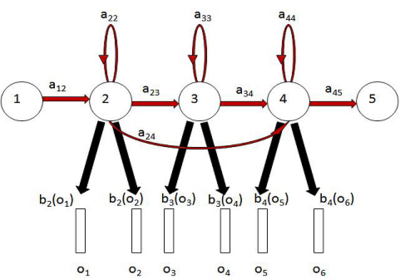
\includegraphics[scale=1.0]{400px-Mfcc_fig5}
    \caption{The Markov Generation Model}
%    \label{fig:mesh1}
\end{figure}


\section{Application of Speech Recognition}

\begin{description}
  \item[$\bullet$ Automation of Operator Services] Systems like the Voice Recognition Call Processing (VRCP) system introduced by AT and T or the Automated Alternate Billing System (AABS) introduced by Nortel enabled operator functions to be handled by speech recognition systems. The VRCP system handled so-called ‘operator assisted’ calls such as Collect, Third Party Billing, Person-to- Person, Operator Assisted Calling, and Calling Card calls. The AABS system automated the acceptance (or rejection) of billing charges for reverse calls by recognizing simple variants of the two word vocabulary Yes and No.
  \item[$\bullet$ Automation of Directory Assistance]  Systems were created for assisting operators with the task of determining telephone numbers in response to customer queries by voice. Both NYNEX and Nortel introduced a system that did front end city name recognition so as to reduce the operator search space for the desired listing, and several experimental systems were created to complete the directory assistance task by attempting to recognize individual names in a directory of as many as 1 million names. Such systems are not yet practical (because of the confusability among names) but for small directories, such systems have been widely used (e.g. in corporate environments).
  \item[$\bullet$ Voice Dialing] Systems have been created for voice dialing by name (so- called alias dialing such as Call Home, Call Office) from AT and T, NYNEX, and Bell Atlantic, and by number (ATandT SDN/NRA) to enable customers to complete calls without having to push buttons associated with the telephone number being called.
  \item[$\bullet$ Voice Banking Services] A system for providing access to customer accounts, account balances, customer transactions, etc. was first created in Japan by NTT (the ANSER System) more than 10 years ago in order to provide a service that was previously unavailable. Equivalent services have been introduced in banks worldwide over the last several years. 
  \item[$\bullet$ Voice Prompter]A system for providing voice replacement of touch-tone input for so-called Interactive Voice Response (IVR) systems was introduced by AT and T in the early 1990’s (initially in Spain because of the lack of touch- tone phones in that country). This system initially enabled the customer to speak the touch-tone position (i.e. speak or press the digit one); over time systems have evolved so that customers can speak the service associated with the touch-tone position (e.g. say reservations or push the 1-key, say schedule or push the 2-key, etc. 
  \item[$\bullet$ Directory Assistance Call Completion] This system was introduced by both AT and T and NYNEX to handle completion of calls made via requests for Directory Assistance. Since Directory Assistance numbers are provided by an independent system, using Text-to-Speech synthesis to speak out the listing, speech recognition can be used to reliably recognize the listing and dial the associated number. This highly unusual use of a speech recognizer to interface with a speech synthesizer is one of the unusual outgrowths of the fractionation of the telephone network into local and long distance carriers in the United State.
  \item[$\bullet$ Reverse Directory Assistance] This system was created by NYNEX:, Bellcore, and Ameritech to provide name and address information associated with a spoken telephone number.Information Services. These type of systems enable customers to access information lines to retrieve information about scores of sportilng events, traffic reports, weather reports, theatre bookings, restaurant reservations, etc. 
  \item[$\bullet$ Agent Technology] Systems like Wildfire and Maxwell (AT and T) enable customers to interact with intelligent agents via voice dialogues in order to manage calls (both in-coming and out-going calls), manage mesaages (both voice and email), get information from the Web (eg, movie reviews, calling directories), customize services (e.g., first thing each morning the agent provides the traffic and weather reports), personalize services (via the agent personality, speed, helpfulness), and adapt to user preferences (e.g., learn how the user likes to do things and react appropriate.
  \item[$\bullet$ Customer Care] The goal of customer care systems is to replace Interactive Voice Response systems with a dialogue type of interaction to make it easier for the user to get the desired help without having to navigate complicated menus or understand the terminology of the place being called for ihelp. The How May I Help You (HMIHY) customer care system of AT and T is an excellent example of this type of system.
  \item[$\bullet$ Computer Telephony Integration] Since the telecommunication network of the future will integrate the telephony (POTS) and computer (Packet) networks, a range of new applications will arise which exploit this integration more fully. One prime example is registry services where the network locates the user and determines the most appropriate way to communicate with them. Another example is providing a user cache of the most frequently accessed people in order to provide a rapid access mechanism for these frequently called numbers.
  \item[$\bullet$ Voice Dictation]  Although the desktop already supports voice dictation of documents, a prime telecommunications application of speech recognition would be for generating voice responses to email queries so that the resulting message becomes an email message back to the sender (rather than a voice mail response to an email message).
\end{description}

\section{Summary}
In this chapter, we describes about the Introduction of Speech Recognition concept. Then further we discussed about Hidden mrkov's Model. In chapter we discussed about advantages of Speech Recognition systems, application of Speeh Recognition System.












\appendix

\chapter{Additional}
Lorem ipsum dolor sit amet, consectetur adipiscing elit, sed do eiusmod tempor incididunt ut labore et dolore magna aliqua. Ut enim ad minim veniam, quis nostrud exercitation ullamco laboris nisi ut aliquip ex ea commodo consequat. Duis aute irure dolor in reprehenderit in voluptate velit esse cillum dolore eu fugiat nulla pariatur. Excepteur sint occaecat cupidatat non proident, sunt in culpa qui officia deserunt mollit anim id est laborum.


\printbibliography

%\bibliographystyle{unsrt}
%\bibliography{sample}

\end{document}

